% status: 100
% chapter: REST

\title{BigData With Benfords Law}

\author{Ravinder Lambadi}
\affiliation{%
  \department{School of Informatics, Computing, and Engineering}
  \institution{Indiana University}
  \city{Bloomington}
  \state{IN}
  \postcode{47408}
  \country{USA}}
\email{rlambadi@iu.edu}


\author{Orly Esteban}
\affiliation{%
  \department{School of Informatics, Computing, and Engineering}
  \institution{Indiana University}
  \city{Bloomington}
  \state{IN}
  \postcode{47408}
  \country{USA}}
\email{esteban@iu.edu}

\begin{abstract}
Analyzing large amount of data detecting for anomalies 
can be a painful endeavor. Not only would you need a 
reliable algorithm to analyze data but also an 
infrastructure to support an ever growing data to 
analyze. This paper attempts to address these concerns. 

It is observed that a lot of real-life data, 
from personal expenses to world population data, 
tend to obey Benford’s Law. Because of this phenomenon, 
Benford’s Law has been leveraged 
in a lot of statistical analysis – including fraud 
detection. In 2009,  Benford’s Law has been utilized 
to detect election fraud in Iran.

In this paper, the authors first determined 
the universality of the law and drew criteria 
where the the law is applicable by citing 
observations made from other source and more 
importantly the authors’ own observations by 
using data from data.gov. The authors then 
created a web service using the law and deployed 
the service to the cloud.

\end{abstract}

\keywords{hid-sp18-514, hid-sp18-506, REST, Benford's Law, Python}

\maketitle

\section{Introduction}
Benford’s law is a phenomenon about the distribution 
of the first-digits of numerical sets of real-life data. 
The law states that the distribution of the first digits
follows a certain mathematical pattern. If the probability 
distribution of the digits is evenly flat, each digit from 
1 thru 9 would appear 11 percent of the time. However, 
with with Bendford’s Law, The probability distribution 
tends to go lower from the digit 1 to the digit 
9~\cite{hid-sp18-514-benfordwiki}.
For example, the digit 1 tends to occur about 30 percentage 
of the time while the digit 9 about 4.6 percentage 
of the time. The chart below shows the frequency of 
leading digits that obey Benford’s Law vs flat even distribution


\begin{figure}[!ht]
\centering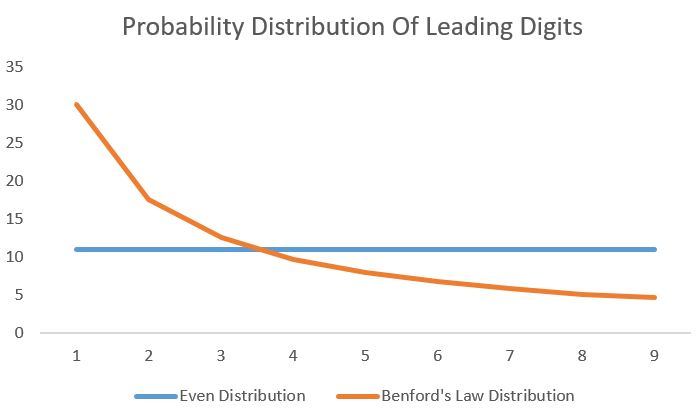
\includegraphics[width=\columnwidth]{images/probability_dist.JPG}
  \caption{Probability distribution of Leading Digits}\label{f:prob-dist-lead}
\end{figure}

Because of this phenomena, Benford’s Law is used in many 
fraud detection algorithms. The Bureau of Internal Revenue 
Service uses this law to catch tax cheats. 
A presidential election fraud was detected in 
Iran in 2009 thru the application of Benford’s Law.


A dataset is said to satisfy Benfords Law if the leading 
digits have the following the probability distribution: 

\begin{figure}[!ht]
\centering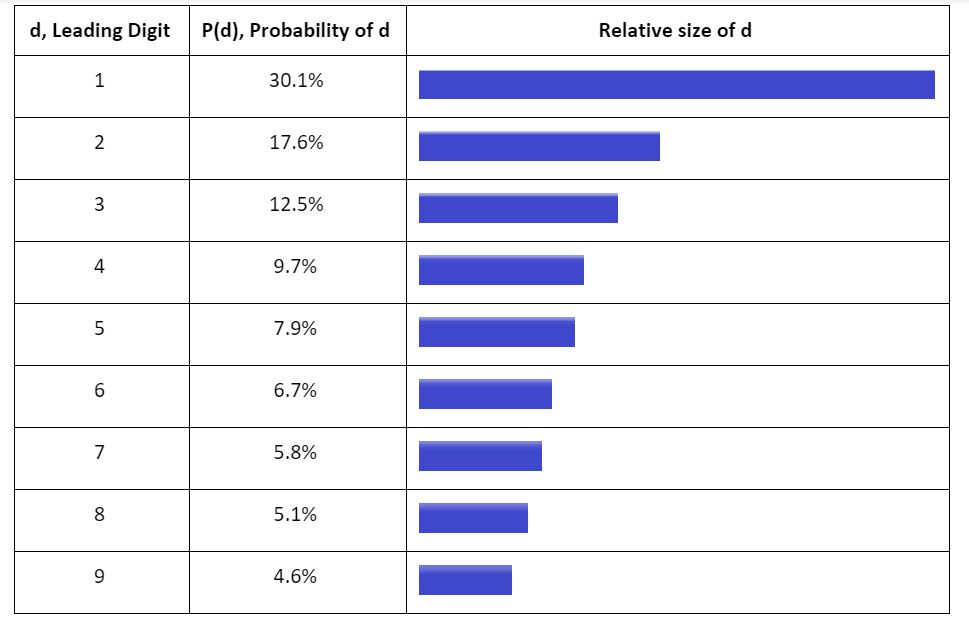
\includegraphics[width=\columnwidth]{images/benfords_law.JPG}
  \caption{Probability distribution of Benfords Law}\label{f:prob-dist-ben}
\end{figure}


In mathematical terms, Benford’s Law can be represented 
by the following equation:

\[P (d) = \log (d+1) - \log (d)\]

Example: In case base 10 is used we obtain the 
probability for the leading digit 1, as

\[P (1) = \log (1+1) - \log (1) = 0.301 \]

which means, if the dataset complies 
with Benford's Law, the probability of finding a 
leading digit 1 is about 30.1 percentage of the time. 
Therefore, Benford’s Law indicates that the most 
likely leading digit for us to see is 1, the second 
most likely 2, the third most 3, the fourth most 
likely 4, and so on.

Some real-life examples of data where Benford’s Law is 
seen in the choice of iPhone passcodes. 
It is determined that most passcodes start with a 1 or  
2 and least with a 9. The yellow bars show the actual
distribution compared to the Benford’s 
Law expected distribution indicated by the 
red triangles~\cite{hid-sp18-514-iphone-benford}

\begin{figure}[!ht]
\centering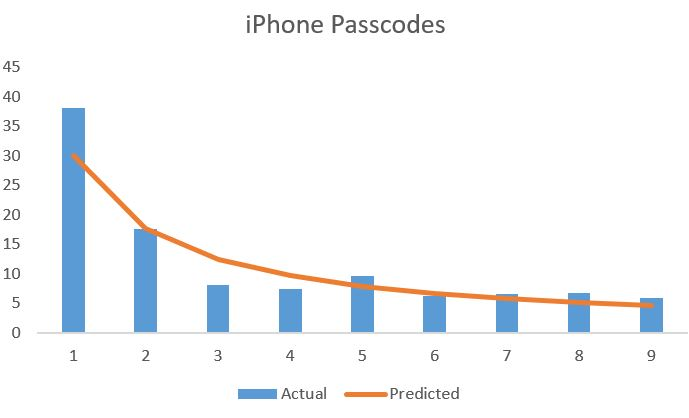
\includegraphics[width=\columnwidth]{images/iphone_benford.JPG}
  \caption{Testing Benford's Law for iPhone Passcodes}\label{f:iphone-pass_ben}
\end{figure}


Another example is the distribution of the first 
digits of the population of more than 200 countries 
in the world as shown in the graph below. 
The red bars show the distribution while 
the black dots show the distribution as 
predicted by Benford’s Law~\cite{hid-sp18-514-benfordwiki}

\begin{figure}[!ht]
\centering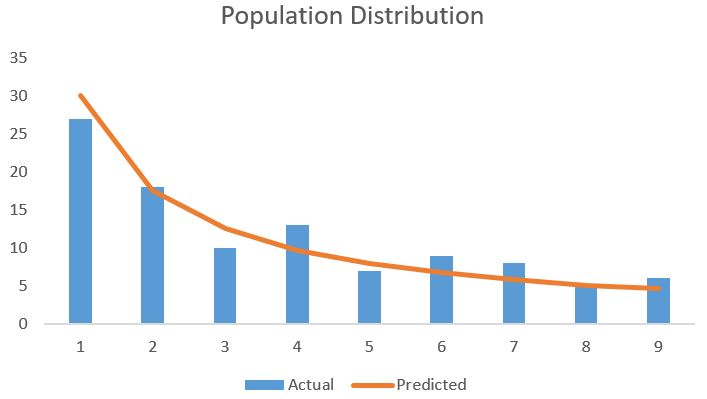
\includegraphics[width=\columnwidth]{images/benford_country.JPG}
  \caption{First Digit Population Distribution}\label{f:pop-dist-countries}
\end{figure}

The logarithmic function can be in any base. 
We have developed a REST service that allows
the calculation of Benford's Law. 
The service will allow us to specify 
the base and the data set as input. 

\section{Objectives}
The popularity and the size of data being 
analyzed using Benford’s Law have lead the authors 
to conduct this study. 
There are 2 objectives that the authors aim to achieve:

\begin{enumerate}
\item
Write a performant web service that takes in numerical datasets. 
The web service should be performant enough to handle large datasets. 
It should take in a URL of the dataset (for this exercise the authors used
large datasets from data.gov). Analyze the data and return a visualization 
of the data side by side with the BL’s predicted distribution.
\item
Deploy the web service to an infrastructure that should be able to handle 
the huge amount of load both in terms of numbers of sessions and the size 
of the data. To ensure that the web service can handle the load, 
the authors deployed the web service in the cloud that use latest 
technology to keep up with the expected load.
\end{enumerate}

\section{Limitations of Benford’s Law}
It is important to note that Benford’s Law assumes that the 
dataset in question is generated randomly. A naturally occurring 
dataset where the numbers generated are intentionally restricted 
is not a fit for Benford’s Law analysis. 

Also when certain rules are applied to generate 
the numbers in the dataset, Benford’s Law may not be applicable.
For example, the social security number is generated with a 
certain formula that applies only to a certain state 
and therefore its leading digit may not be truly random. 

Because of this limitations, before Benford’s Law is
used in controversial investigations, the auditor must 
first determine if the numbers are truly randomly generated, 
of large orders of magnitude and its size is big enough 
to draw reliable conclusions.

The adequate sample size for BL is not exactly 
determined. However,this source 
(Kenny, D.A. 2015. Measuring model fit, 
available from~\cite{hid-sp18-514-Kenny-Measuring-model}
[Accessed January 2017].)  
claims that the consensus is at least 50-100 minimum data 
points for BL to be perceived. The authors are not 
comfortable with this limit but would recommend at least 
a thousand data points. The general rule is that more 
data points the more reliable the results would be.

\section{REST Services To Determive Benfords's Law}

There are four universal services have been built to determine
whether the provided data set follows Benford’sfords's law.

\begin{enumerate}
 \item computeBenfordLawWebDataSetService
 \item downloadDataSet
 \item computeBenfordLawCSVDataSet
 \item computeBenfordLawExcelDataSet
\end{enumerate}

\subsection{computeBenfordLawWebDataSetService - REST API}
computeBenfordLawWebDataSetService is 
a REST API to defect fraud using Benford's Law.
We have taken dataset from~\cite{hid-sp18-514-aust-cc-benford}
to verify benford law.

This dataset has 690 credit card customers.
There are chances that few fraudulent customer 
applications got approved due to errors. 
This service will find some possible frauds using 
Benford's law so that the bank can perform
further investigation.

There are no column names defined in the original dataset.
so the authors defined the column names as:
A1 to A15. Using Pandas library this dataset
is imported and created the dataframe.

Last column A15 is a numerical field 
indicates whether credit card is approved. 
1 indicates approved and 0 indicates didn't 
get approved.

To test the service, pass the below query
parameter-column:A2 to the API.


After analysis of the figure generated 
by the service, noticed that the bars 
for digits 3,4,5,6,7 are not within 
Benford's law prediction. 
All of them are above Benford's law 
line which means that this bar deviated 
from Benford's law. 
Therefore, this should trigger an investigation 
to confirm wheter or not the customers committed fraud. 

\begin{figure}[!ht]
\centering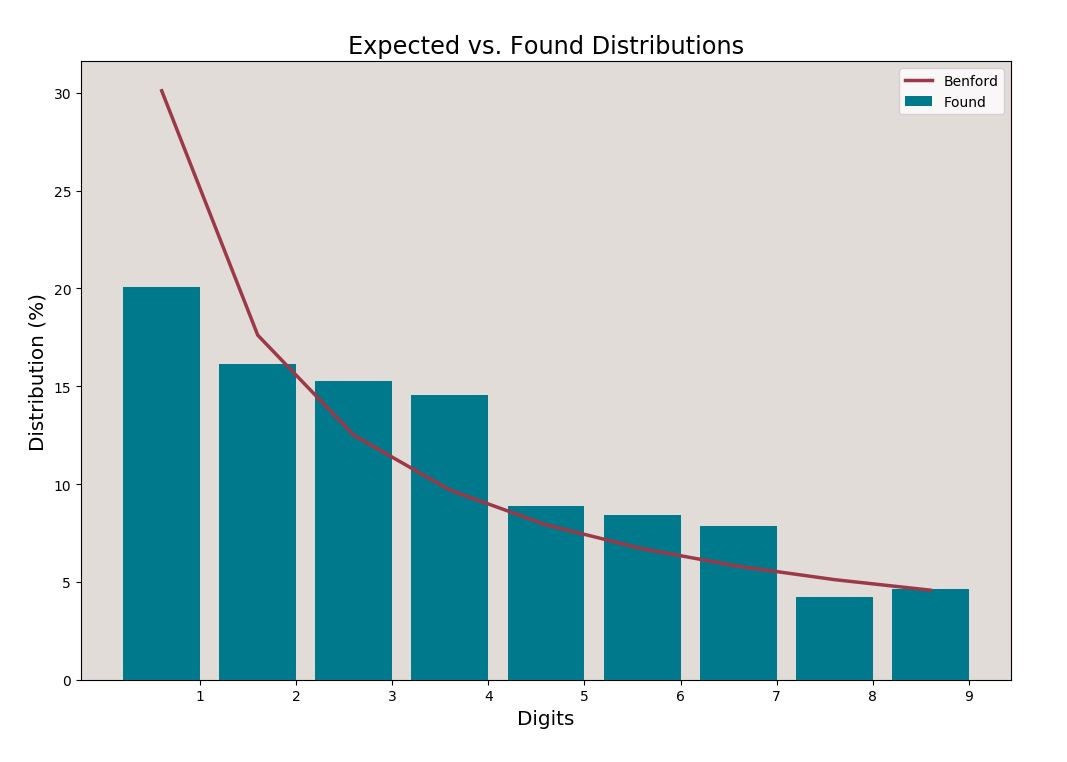
\includegraphics[width=\columnwidth]{images/fraudDet_cc_data.JPG}
  \caption{Credit Card Application Dataset}\label{f:aust-cc-data}
\end{figure}


\subsection{downloadDataSet - REST API}
downloadDataSet is a REST API service tested on 
on-premise and cloud environment. This service requires two 
input paramaters to download the dataset.

Below parameters need to pass to this REST API:

\begin{enumerate}
\item dataLocation - Location of the dataset. 
 Ex:~\cite{hid-sp18-514-excelDatalocation}
\item fileName - Dataset file name to be downloaded 
 as, Ex: nsn-extract.xlsx
\end{enumerate}


\subsection{computeBenfordLawExcelDataSet - REST API}
computeBenfordLawExcelDataSet is a REST API service tested on 
on-premise and cloud environment. This service requires two 
input paramaters to determine Benfords's Law. This service
process and send back the output 
for all excel based datasets.

Below parameters need to pass to this REST API:

\begin{enumerate}
\item columnName - Name of the column in the 
 dataset for which Benford Law determation required. 
 Ex: Price
\item fileName - Dataset file name to be downloaded 
 as, Ex: nsn-extract.xlsx
\end{enumerate}

\subsection{computeBenfordLawCSVDataSet - REST API}
computeBenfordLawCSVDataSet is a REST API service 
tested on on-premise and cloud environment. 
This service requires two input paramaters to 
determine Benfords's Law. This service
process and sends back the output 
for all CSV and Text based datasets.

Below parameters need to pass to this REST API:

\begin{enumerate}
\item columnName - Name of the column in the 
 dataset for which Benford Law determation required. 
 Ex: COUNT PUBLIC ASSISTANCE TOTAL
\item fileName - Dataset file name to be downloaded 
 as,Ex: DemographicStatistics.csv
\end{enumerate}

\subsection{Benfords Law Verification for National Stock 
Number Datset - Excel}
National Stock Number extract dataset downloaded from 
~\cite{hid-sp18-514-nsn-ds-desc} to verify benfords law.

BenfordLawExcelDataSetService returns the below
output for the dataset~\cite{hid-sp18-514-excelDatalocation}
and columns name was:Price.

\begin{figure}[!ht]
\centering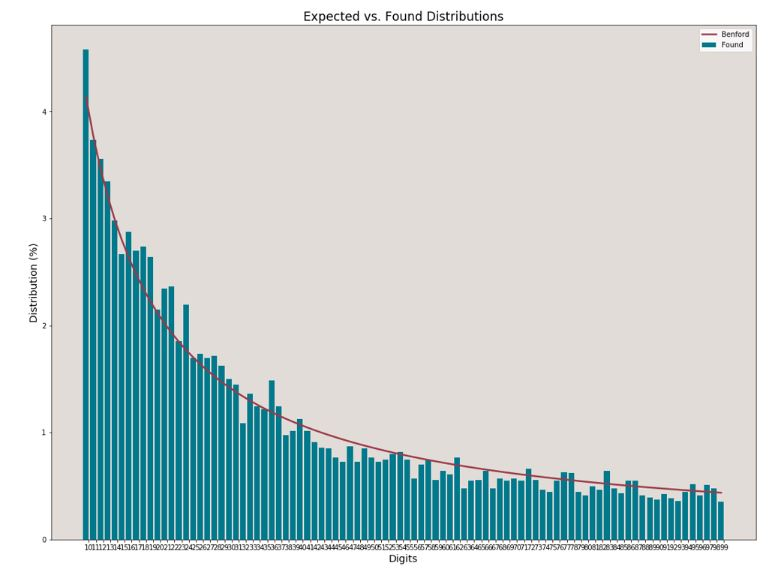
\includegraphics[width=\columnwidth]{images/benford_nsn.JPG}
  \caption{Benfords Law Verification for - NSN DS}\label{f:NSN-ds-benfordlaw}
\end{figure}

The line is Benford’s Law prediction and the bars are 
the actual data. This dataset follows the benford's law
because most of the bars are within the benford's law prediction.


\subsection{Credit card transactions Dataset}
This dataset contains card transactions downloaded 
from~\cite{hid-sp18-514-purchase-card-desc}
for Benford's Law verification.

BenfordLawCSVDataSetService returns the below
output for the dataset~\cite{hid-sp18-514-purchase-card-ds}

\begin{figure}[!ht]
\centering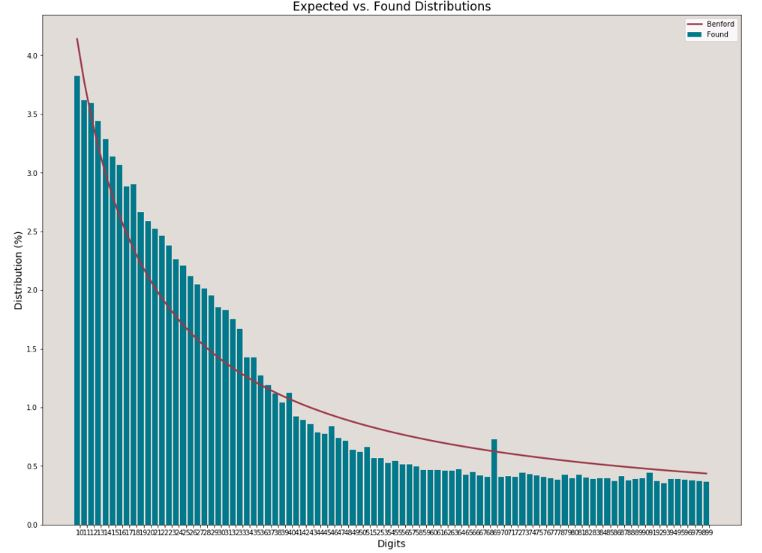
\includegraphics[width=\columnwidth]{images/ben_card_trx.JPG}
  \caption{Fraud Detection Using Benford Law}\label{f:card-ds-benfordlaw}
\end{figure}

The line is Benford’s Law prediction and the bars are 
the actual data. This dataset does not follow the benford's law
because most of the bars are outside the benford's law prediction.


\section{Further Analysis Needed}
The results drawn from these examples should 
be analyzed with great caution. They should 
never be used as an absolute proof of presence 
or absence of manipulation. A clever fraud who 
is familiar with the law can still manipulate 
the data that remain undetectable with the 
application of Benford’s Law.

However, we should not easily dismiss the results 
when comparing the data with Benford’s Law. 
A good fitness test must be conducted to determine 
how the data conforms with Benford’s Law.
For the goodness of fit test, the following can be implemented:

\begin{enumerate}
\item A visual graph of the actual data distribution 
layed on top of the expected Benfords Law distribution
\item Root mean square error fit index.
\item Chi-square goodness of fit test. Although, 
this is sensitive to sample sizes and outliers.
\end{enumerate}

The level of significance for chi-square test 
but a widely acceptable confidence level is 95 percentage

\section{DataSet - Accuracy For Benford's Law Prediction}
Authors verified three datasets in this paper. Only one
date set - National Stock Number extract 
complied the Benford's Law.

\section{Conclusion}
This paper has shown the Benford’s Law is observed in 
the the real life data in data.gov and in many other 
cited studies. Given that Benford’s Law is gaining prominence 
and as data sizes explode, there is a need for effective scanning
of the data to identify conformity the with Benford’s Law. 
The authors have successfully set up this mechanism to 
keep up with the expected load.


Benford’s Law can recognize the probabilities of highly  
likely or highly unlikely frequencies of numbers in a data set.
The probabilities are based on mathematical logarithms of the 
occurrence of digits from the given data sets for Benford's 
validity. We have verified Benford law for stock price 
dataset and fraud detection on card transactions.
The limitation with Benford Law is, it performs 
Benford Law analysis on Numeric data type column only. 
And for accurate analysis it requires large dataset. 
For smaller dataset the analysis might not accurate.

As seen in the results above, the Law tends to 
apply the most to data that are uniformly 
distributed across several orders of magnitude. 
It may not apply if the range of values are 
very tight. The credit card transaction above 
is way off Benford’s Law prediction. 
This should prompt further investigation 
since credit card transactions are usually 
in orders of several magnitude. 
It’s either the transaction are purposely 
fraudulent or unintentionally filled 
with bad data or it is one of 
the few exceptions where Benford’s Law does not apply.


\bibliographystyle{ACM-Reference-Format}
\bibliography{report} 
